\documentclass[cp1251%,draft % раскомментировать, если нужен черновой режим
               ]{jetp} % jetp.cls
\usepackage{amsbsy}
%\usepackage{epstopdf}
%% Преамбула %%%%%%%%%%%%%%%%%%%%%%%%%%%%%%%%%%%%%%%%%%%%%%%%%%%%%%%%%%%
\twocolumn % закомментировать, если не нужен двухколоночный вариант
%%%%%%%%%%%%%%%%%%%%%%%%%%%%%%%%%%%%%%%%%%%%%%%%%%%%%%%%%%%%%%%%%%%%%%%%
%%%%%%%%%%%%%%%%%%%%%%%%%%%%%%%%%%%%%%%%%%%%%%%%%%%%%%%%%%%%%%%%%%%%%%%%
%\usepackage[intlimits]{amsmath}
%\usepackage{amssymb,amsfonts}

\usepackage[T2A]{fontenc}
\usepackage[cp1251]{inputenc}
\usepackage[english,russian]{babel}
\usepackage{epstopdf}
\usepackage[autostyle]{csquotes}

\usepackage{cuted}   
\usepackage{lipsum}  

\usepackage[intoc,nocfg,russian]{nomencl}
\newcommand{\nomencl}[2]{#1 --- #2\nomenclature{#1}{#2}}
\setlength{\nomlabelwidth}{3em}
\setlength{\nomitemsep}{-\parsep}
\setcounter{tocdepth}{2}
\renewcommand{\nomlabel}[1]{#1 ---}
\makenomenclature

\usepackage{wrapfig}
\let\vec=\mathbf
%\graphicspath{{fig/}}
\def\mprp{\mbox{\tiny $\bot$}}
\def\mprl{\mbox{\tiny $\|$}}
\def\th{\mbox{th}}

\def\D{\mathrm{d}}
\def\beq{\begin{eqnarray}}
\def\eeq{\end{eqnarray}}
\def\ee{\varepsilon}
\def\lm{\lambda}
\newcommand{\prp}[1]{#1_{\mbox{\tiny $\bot$}}}
\newcommand{\pprl}[1]{#1_{\mbox{\tiny $\|$}}}
\newcommand{\ii}{\mathrm{i}} % мнимая единица
\newcommand{\dd}{\mathrm{d}} % дифференциал
\newcommand{\eee}{\mathrm{e}} % основание натуральных логарифмов
\def\HH{H\!\!\left(\frac{4 m^2}{\pprl{q}^2}\right)}
\def\HHi{H\!\!\left(\frac{4 m^2}{\pprl{q'^2}}\right)}
\def\HHii{H\!\!\left(\frac{4 m^2}{\pprl{q''^2}}\right)}
\def\ggg{\gamma \rightarrow \gamma \gamma}
\def\ff{\Lambda}
\def\tff{\widetilde \Lambda}
\def\1{1 \to 1 \, 2}
\def\2{1 \to 2 \, 2}
\def\S{S}
\def\J{{\cal J}}
\def\A{{\cal A}}
\def\P{{\cal P}}
\def\M{{\cal M}}
\newcommand{\bs}{\boldsymbol}

\begin{document}

%%%%%%%%%%%%%%%%%%%%%%%%%%%%%%%%%%%%%%%%%%%%%%%%%%%%%%%%%%%%%%%%%%%%%%%%

\title{Резонансное комптоновское рассеяние в замагниченной среде}

%% ---------------------------------------------------------------------
%% Пример:
%% \affiliation{Физический институт им.~П.~Н.~Лебедева Российской
%% академии наук\\ 119991, Москва, Россия}
%% ---------------------------------------------------------------------

\author{Д.~А.}{Румянцев}
\email{rda@uniyar.ac.ru} % электронный адрес
%% ---------------------------------------------------------------------
%% Примеры: \email{i.i.ivanov@yandex.ru}
%%          \email{i.i.ivanov@yandex.ru, ivanovii@gmail.com}
%% ---------------------------------------------------------------------
\affiliation{Ярославский государственный университет им. П.Г. Демидова\\
150000, Ярославль, Россия}

\author{А. А.}{Ярков}
\email{a121@mail.ru} % электронный адрес
\affiliation{Ярославский государственный университет им. П.Г. Демидова\\
150000, Ярославль, Россия}

\affiliation{Ярославское высшее военное училище противовоздушной обороны\\
150001, Ярославль, Россия}

\author{Д.~М.}{Шленев} % второй автор и так далее
\affiliation{Ярославское высшее военное училище противовоздушной обороны\\
150001, Ярославль, Россия}
% \affiliation{} % второе место работы и так далее
\email{allen\_caleb@rambler.ru}


%% ---------------------------------------------------------------------
%% Примеры: \email{i.i.ivanov@yandex.ru}
%%          \email{i.i.ivanov@yandex.ru, ivanovii@gmail.com}
%% ---------------------------------------------------------------------


\rtitle{Резонансное комптоновское рассеяние...}
\rauthor{Д.~А.~Румянцев, А.~А.~Ярков, Д.~М.~Шленев}


\abstract{
Рассмотрен резонансный процесс  комптоновского рассеяния в сильном магнитном поле. Получена вероятность реакции 
в зависимости от энергии и углов распространения начальных частиц. Вычислен коэффициент поглощения 
фотона за счет процесса в пределе сверхсильных магнитных полей. Найдены границы по энергиям начального фотона, в которых приближение узкого резонансного пика будет находиться в согласии с результатами, полученными для пика конечной ширины.
}

\maketitle
%%%%%%%%%%%%%%%%%%%%%%%%%%%%%%%%%%%%%%%%%%%%%%%%%%%%%%%%%%%%%%%%%%%%%%%%
%% Текст статьи %%%%%%%%%%%%%%%%%%%%%%%%%%%%%%%%%%%%%%%%%%%%%%%%%%%%%%%%
%%%%%%%%%%%%%%%%%%%%%%%%%%%%%%%%%%%%%%%%%%%%%%%%%%%%%%%%%%%%%%%%%%%%%%%%

\section{Введение}

Интерес к изучению комптоновского рассеяния $\gamma e \to \gamma e$ в 
сильном магнитном поле ($B\gtrsim B_e = m^2 / e= 4.41\cdot 10^{13}$ Гс~\footnote{В данной работе используется естественная система единиц: $c = \hbar = k_{\rm{B}} = 1$, $m$ -- масса электрона, $e > 0$ -- элементарный заряд.}) первоначально был вызван неожиданным открытием циклотронных 
спектральных линий у двойных рентгеновских 
пульсаров~\cite{Truemper1978,Makishima1990,Grove1995}, которые изначально 
интерпретировались либо как циклотронное поглощение, либо как циклотронное 
излучение~\cite{Truemper1978}. Дальнейшее повышение разрешения детекторов по 
энергии позволило уверенно заключить, что циклотронные особенности связаны 
именно с резонансным поглощением фотона~\cite{Mihara:1990}.
При этом под циклотронным резонансом обычно понимается 
резкое увеличение сечения рассеяния по сравнению с классическим томсоновским 
сечением, $\sigma_T = 8 \pi \alpha^2 /(3 m^2)$. В одной из первых 
работ по этой тематике~\cite{Canuto:1971} выражение для сечения комптоновского рассеяния в магнитном поле без плазмы было получено в нерелятивистском пределе, и для фотона, распространяющегося вдоль магнитного поля, в сечении был обнаружен резонансный пик при энергии: 
\begin{equation}\label{eq:w_B}
	\omega_B\simeq \frac{\beta}{m}\, ,
\end{equation}
 %
\noindent где введено обозначение $\beta = eB$.

Кроме того, в работе~\cite{Canuto:1971} также было показано, что сечение рассеяния фотона 
на электроне
значительно зависит как от поляризационного состояния фотона, так и от угла 
между направлением импульса начального фотона и направлением магнитного поля. В 
последовавшей за ней 
статье~\cite{Gnedin1973} 
исследовалось изменение энергии фотона в комптоновском процессе, кратное 
циклотронной частоте $\omega_B$. 
В следующих работах~\cite{Borner1979,Ventura:1979} 
были получены результаты для полного сечения рассеяния фотона на электроне с использованием формализма работы~\cite{Canuto:1971}. Тем не менее эти результаты будут справедливыми только для относительно слабого магнитного поля~$B\lesssim10^{12}$~Гс. Однако при значениях магнитного поля~$B>10^{12}$~Гс, как было показано в работах~\cite{Herold:1979,Melrose:1983III},   учет релятивистских эффектов в сечении комптоновского рассеяния становится 
существенным.

В представленных выше работах предполагалось, что начальный и конечные электроны находятся 
на основном уровне Ландау, что является справедливым для предела сверхсильного магнитного поля $B\gg B_e$
и/или низких температур $T\ll m$. В этом случае резонансный 
пик~(\ref{eq:w_B})  смещается в область более низких энергий фотона, а кроме 
него также возникает бесконечный ряд резонансных пиков, соответствующих разным 
уровням Ландау $n=0,1,\dots$ 
виртуального электрона. Эти пики реализуются при энергиях фотона~\cite{Daugherty:1986}:
\begin{equation}\label{eq:whn}
	\omega_n(\theta)= \frac{\sqrt{m^2+2 \beta n \sin^2\theta} - 
		m}{\sin^2\theta}\, ,
\end{equation}
где $\theta$ -- угол между импульсом начального фотона и направлением 
магнитного поля. 

С другой стороны, в результате комптоновского процесса могут возбуждаться 
высшие уровни Ландау начального электрона, что, в свою очередь, может выступать 
механизмом рождения фотонов малых энергий для магнитных полей $B\lesssim 
B_e$~\cite{Daugherty:1986,Bussard:1986}. В таком случае для произвольного уровня Ландау $\ell$ 
начального электрона резонансные пики будут наблюдаться на энергиях:

\begin{equation}\label{eq:resAll}
	\omega_{n\ell}(\theta)=\frac{\sqrt{M_\ell^2 - \sin^2\theta (M_\ell^2-M_n^2)}-M_\ell}{\sin^2\theta}\, ,
\end{equation}
где $M_\ell=\sqrt{m^2+2\beta \ell}$, $M_n=\sqrt{m^2+2\beta n}$.

В рассмотренных выше работах сечение комптоновского рассеяния 
становится бесконечным при энергиях фотона, соответствующих циклотронным 
резонансам~(\ref{eq:whn}) вследствие предположения о 
большом времени жизни виртуальных частиц. По этой причине их результаты 
справедливы только для областей энергий фотона вдали от резонансов
и могут быть применены, например, для моделирования излучения 
замагниченной 
	холодной плазмы вблизи поверхности нейтронных 
	звезд~\cite{Ozel:2001} или же для относительно слабых магнитных 
	полей $B\lesssim 10^{10}$ Гс~\cite{Zavlin:1996}.

С другой стороны, учет резонансов в комптоновском процессе является необходимым 
при моделировании спектров излучения сильно замагниченных нейтронных 
звезд~\cite{Alexander:1991,Araya:1999,Ho:2001,Lyutikov:2006,Potekhin:2004,Schonherr:2007,Nishimura:2008,Suleimanov:2009}.
При этом вблизи поверхности нейтронной звезды, где формируется излучение, резонансный 
обратный комптоновский процесс рассеяния фотонов малых энергий на высокоэнергетических электронах 
является доминирующим процессом, который приводит к охлаждению плазмы 
внутренней магнитосферы и образованию высокоэнергетического хвоста в спектре 
излучения~\cite{Fernandez:2007,Nobili:2008,Baring:2018,Beloborodov:2013}.

Вблизи циклотронных резонансов для расчета сечения комптоновского рассеяния требуется учесть полную 
ширину изменения состояния электрона. Как было показано в работе~\cite{Canuto:1971}, в нерелятивистском пределе присутствует лишь одна резонансная частота, определяемая соотношением~(\ref{eq:whn}), и сечение рассеяния
не зависит от поляризационного состояния электрона (или его спинового состояния), и можно ввести полную ширину, как это было сделано в работе~\cite{Daugherty:1989}. Однако в сильных магнитных полях~$B\gtrsim B_e$ и при высоких энергиях частиц требуется учитывать релятивистские поправки, что приводит к тому, что выражение для сечения становится очень громоздким, поскольку оно имеет бесконечное число резонансов (см.~(\ref{eq:resAll})), содержащихся в сумме по всем промежуточным виртуальным состояниям.

Изначально для учета конечных резонансных пиков использовались усредненные по спину ширины распада промежуточного состояния~\cite{Gonthier:2000, Holodov:2000}. 
Как было указано в работе~\cite{Gonthier:2014}, такой подход не является 
точным, поскольку усреднение по спину некорректно учитывает спиновую 
зависимость времени распада виртуального электрона, что приводит к неверному значению сечения комптоновского рассеяния в точке 
резонанса. Этот недостаток был устранен в работе~\cite{Mushtukov:2016}, где 
представлено сечение рассеяния процесса $\gamma e\to \gamma e$ с учетом 
ширины распада виртуальных промежуточных состояний, которая 
зависит от 
поляризационного состояния электрона. 
Однако полное сечение комптоновского рассеяния, полученное таким методом, 
представляет собой громоздкое выражение, что, например, затрудняет его 
использование в моделях переноса излучения. 

В ряде случаев выражение сечения рассеяния можно упростить для получения аналитического решения различных задач. 
Так, в работе~\cite{Gonthier:2000} была использована аппроксимация сечения рассеяния с учетом резонанса в ультрарелятивистском пределе для случая относительно сильного магнитного поля $B>0.1 B_e$. В точке циклотронного резонанса виртуальный электрон становится реальным и распадается на масштабе комптоновского времени, поэтому вероятность комптоновского рассеяния сводится к вероятности одновершинного процесса поглощения фотона электроном 
$\gamma e \to e$. В работе~\cite{Harding:1991} исследовался вопрос аппроксимации комптоновского сечения с помощью одновершинного процесса поглощения фотона электроном для магнитных полей $B\sim 0.1B_e$. При этом различие между одновершинным процессом поглощения и комптоновским рассеянием становится существенным на высших циклотронных резонансах из-за нерезонансного вклада. Еще один подход рассмотрен в работе~\cite{Rumyantsev:2017}, он заключается в том, что пропагатор виртуального электрона можно заменить на дельта-функцию, когда основной вклад 
в сечение рассеяния будут давать области вблизи резонансов (приближение узкого пика). 

В настоящей работе вычисляется вероятность и дифференциальное сечение рассеяние резонансного комптоновского процесса в приближении узкого резонансного пика в относительно сильном магнитном поле с величиной индукции порядка критического значения $B_e$. Для сверхсильных магнитных полей $B \gg B_e$ вычислена вероятность процесса с учетом конечной ширины изменения состояния электрона.

Статья организована следующим образом. В разделе 2 вычисляется дифференциальное сечение рассеяния электрона на фотоне при резонансе на виртуальном электроне в приближении узкого резонансного пика. Результаты сравниваются с расчетами, полученными с учетом конечной ширины резонансного пика. В разделе 3 вычислена вероятность резонансного комптоновского рассеяния в пределе сверхсильного магнитного поля. В заключении приведены основные результаты статьи.


%%%%%%%%%%%%%%%%%%%%%%%%%%%%%%%%%%%%%%%%%%%%%%%%%%%%%%%%%%%%%%%%%%%%%%%%%%%%%%%%%%%%%%%%%%%%%%%%%%%%%%%%%%%%%%%%%%%%%%%%%%%%%%%%%%%%%%%%%%%%%%%%%%%%%%%%%%%



\section{Вероятность комптоновского рассеяния при резонансе на виртуальном электроне}

Для решения рассматриваемой задачи будем использовать лагранжиан взаимодействия электрона, описываемого волновой функцией $\Psi (X)$, с фотоном в поляризационном состоянии $\lambda$, заданным $A^{(\lambda)}_\mu (X)$,  который имеет следующий вид:
%
\begin{equation}\label{eq:L}
	{\cal L}(X) \, = \,- e [\bar \Psi (X) \gamma^{\mu} A^{(\lambda)}_\mu (X) 
	\Psi(X)] \, ,
\end{equation}
%
\noindent где $V = L_x L_y L_z$ -- нормировочный объем. Волновые функции электрона $\Psi (X)$ в данной работе выбираются как собственные векторы ковариантого оператора~$\mu_z$, который строится следующим образом~\footnote{Обоснование выбора этого метода, предложенного А.А. Соколовым и И.М. Терновым~\cite{Sokolov:1968}, приведено в работе~\cite{Rumyantsev:2017}.}: 
\begin{equation}\label{eq:muz}
	\mu_z=m \Sigma_z - i \gamma_0\gamma_5\left[\vec{\Sigma}\times 
	\vec{P}\right]_z\, ,
\end{equation}
%
\noindent где $\bs\Sigma = - \gamma_0 \bs\gamma \gamma_5$ -- трехмерный оператор спина, $\vec{P} = -i \vec{\nabla} +e \vec{A}$, $A^\mu=\left(0,0,xB,0\right)$ -- 4-вектор потенциала электромагнитного поля в калибровке Ландау.

Уравнение для собственных функций оператора~(\ref{eq:muz}) имеет следующий вид:
\begin{equation}
	{\mu}_z \Psi^s_{p,n}(X)=s M_n \Psi^s_{p,n}(X)\, ,
\end{equation}
в котором квантовое число $s=\pm 1$ определяет поляризационные состояния электрона в постоянном однородном магнитном поле. 
Состояние электрона характеризуется энергией $E_n = \sqrt{p_z^2+M_n^2}$ и является бесконечно вырожденным по $p_z$ и дважды вырожденным по $s$, кроме состояния 
$n=0$, где возможно лишь состояние с $s=-1$. Собственные функции оператора~(\ref{eq:muz}) могут быть представлены следующим образом:
\begin{eqnarray}
\label{eq:psie}
\Psi^s_{p,n}(X) = \frac{e^{-\ii(E_{n} X_0 - p_y X_2 - p_z X_3)}\; U^s_{n} (\xi)}
{\sqrt{4E_{n}M_n (E_{n} + M_n)(M_n + m) L_y L_z}} \, ,  
\end{eqnarray}
где 
\begin{equation}
	\xi(X_1)=\sqrt{\beta}\left(X_1+ \frac{p_y}{\beta}\right)\, .
\end{equation}

Биспиноры  $U^s_{n} (\xi)$ имеют следующий вид:

\beq
\label{eq:U--}
&&U^{-}_{n} (\xi) = \left ( 
\begin{array}{c}
	-\ii\sqrt{2\beta n} \, p_z V_{n-1} (\xi)\\[2mm]
	(E_n + M_n)(M_n + m) V_n (\xi)\\[2mm]
	-\ii\sqrt{2\beta n} (E_n + M_n) V_{n-1} (\xi)\\[2mm]
	-p_z (M_n + m) V_n (\xi)
\end{array}
\right )  ,   
%
\\ [3mm]
\label{eq:U+-}
&&U^{+}_{n} (\xi) = \left ( 
\begin{array}{c}
	(E_n + M_n) (M_n + m) V_{n-1} (\xi)\\[2mm]
	-\ii\sqrt{2\beta n} \, p_z V_n (\xi)\\[2mm]
	p_z (M_n + m) V_{n-1} (\xi)\\[2mm]
	\ii \sqrt{2 \beta n} (E_n + M_n) V_n (\xi)
\end{array}
\right )\! .
\eeq

$V_n(\xi)$ -- нормированные функции гармонического осциллятора, которые 
следующим образом выражаются через полиномы Эрмита $H_n(\xi)$ \cite{Gradstein:1963}:
%
\begin{eqnarray}
\label{eq:V_n}
V_n (\xi) = \frac{\beta^{1/4}\eee^{-\xi^2/2}}{\sqrt{2^n n! \sqrt{\pi}}} \, H_n(\xi)\, .
\end{eqnarray}

Волновая функция фотона $A^{(\lambda)}_\mu (X)$ используется в виде плосковолновых решений:
%
\begin{eqnarray}
	\label{eq:j_k}
	A^{(\lambda)}_\mu (X) = \frac{e^{-\ii(qX)}}{\sqrt{2\omega V}} \, \varepsilon^{(\lambda)}_\mu(q) \, ,
\end{eqnarray}
\noindent где  $q^\mu = (\omega, \vec{q})$ -- 4-вектор энергии-импульса и $\varepsilon^{(\lambda)}_\mu(q)$ -- вектор поляризации фотона. В замагниченной плазме с нулевым химическим потенциалом у фотона есть два возможных поляризационных состояния~\footnote{Подробный анализ дисперсионных свойств фотона в замагниченной среде можно найти в работе~\cite{Chistyakov:2009} и цитированных в ней статьях.}, которые определяются следующими векторами поляризации:
%
\begin{eqnarray}
\ee_\alpha^{(1)}(q) = \frac{(q \varphi)_\alpha}{\sqrt{q_{\mprp}^2}},
\qquad
\ee_\alpha^{(2)}(q) = \frac{(q \tilde \varphi)_\alpha}
{\sqrt{q_{\mprl}^2}} \, ,
\label{epsilon}
\end{eqnarray}
%
\noindent где $\varphi_{\mu \nu} =  F_{\mu \nu} /B$ -- обезразмеренный тензор электромагнитного поля и ${\tilde \varphi}_{\mu \nu} = \frac{1}{2}\varepsilon_{\mu \nu \rho \sigma} \varphi_{\rho \sigma}$ -- тензор, дуальный к нему, а также введены обозначения $q_{\mprl}^2 = \omega^2 - q_z^2$ и $q_{\mprp}^2 = q_x^2 + q_y^2$.

$S$-матричный элемент рассеяния фотона поляризации $\lambda$ на электроне в поляризационном состоянии $s$, находящемся на уровне Ландау $\ell$, с рождением электрона в поляризационном состоянии $s^{\, \prime}$ на уровне Ландау $\ell'$ и фотона поляризации $\lambda'$ с учетом лагранжиана~(\ref{eq:L}) может быть представлен в виде:  
%
\beq                          
\nonumber
S^{s^{\, \prime} s}_{\gamma^{(\lambda)} e \to \gamma^{(\lambda')} e'} 
&=& - e^2\int \dd^4 X \dd^4 Y A^{(\lambda)}_\mu (X) A^{(\lambda')}_{\mu'} (Y)
\times 
\\[3mm]
\nonumber
&\times& 
\, \left [\bar \Psi^{s'}_{p',\ell'}(Y) \gamma_{\mu'} 
S (Y,X) 
\gamma_\mu \Psi^{s}_{p,\ell}(X) \right ]\, +
\\[3mm]
\label{eq:S1a}
&+& (A^{(\lambda)}_\mu, \gamma_\mu \leftrightarrow A^{(\lambda')}_{\mu'}, \gamma_{\mu'})\, .
\eeq

Входящий в него пропагатор $S(X,Y)$ удобно рассматривать в виде разложения по уровням Ландау:
\begin{equation}
	S(X,Y) = \sum_{n=0}^{\infty}\sum_{s''=\pm 1} S_n^{s''} (X,Y)\, .
\end{equation}

Вклад в разложение пропагатора от уровня Ландау $n$ и поляризационного состояния $s''$ можно представить следующим образом:
%
\begin{eqnarray}
\label{eq:propagator}
S^{s''}_n (X, Y) && =  \int \frac{\dd p_0 \dd p_y \dd p_z}{(2\pi)^3} \times
\\[3mm]
\nonumber
&& \times \frac{\eee^{- \, \ii \,  p_0 \,(X_0 - Y_0) + 
		\ii p_y \,(X_2 - Y_2) +  \ii \,  p_z \,(X_3 - Y_3)}}
{p_0^2 - p_z^2 - M_n^2 + \ii\, {\cal I}^{s''}_\Sigma (p)} \times
\\[3mm]
\nonumber
&& \times
\, \phi^{s''}_{p, n} (X_1) \bar \phi^{s''}_{p, n} (X'_1) \, ,
\end{eqnarray}
%
\noindent где введено обозначение:
%
\begin{eqnarray}
\phi^{s''}_{p, n} (X_1) =   \frac{U^{s''}_{n} [\xi(X_1)]}
{\sqrt{2 M_n (E_{n} + M_n)(M_n + m)}} \, .
\label{eq:phi_psi}
\end{eqnarray}

${\cal I}^{s''}_\Sigma (p)$ в выражении~(\ref{eq:propagator}) является мнимой частью массового оператора электрона. Резонанс на виртуальном фермионе будет наблюдаться, когда в знаменателе пропагатора~(\ref{eq:propagator}) реальная часть обращается в ноль. Тогда виртуальная частица становится реальной, то есть приобретает определенный закон дисперсии. Анализ кинематики показывает, что это возможно только тогда, когда виртуальный фермион занимает один из высших уровней Ландау, $n > 0$. Частица при этом является нестабильной, и время ее жизни, в нерезонансной области предполагающееся бесконечно большим, определяется мнимой частью массового оператора,  ${\cal I}^{s''}_\Sigma (p)$, учет которой становится необходимым. Она может быть получена с помощью оптической теоремы и представлена в следующем виде~\cite{Weldon:1982, Zhukovski:1994}:
%
\begin{eqnarray}
{\cal I}^{s''}_\Sigma (p) = - \frac{1}{2}\, p_0 \; \Gamma_n^{s''} \, ,
\label{eq:I_Sigma}
\end{eqnarray}
\noindent где $\Gamma_n^{s''}$ -- полная ширина изменения состояния электрона
за счет процесса рассеяния фотона на электроне, 
которую можно выразить через ширину поглощения электрона в процессе $e_n \to \gamma^{(\lambda')
e_{\ell'} }$~\cite{Weldon:1983}:
\begin{eqnarray}
	\label{Gns}
	\Gamma_n^{s''} \simeq 
	\Gamma^{(abs) \, s''}_{e_n  \to \gamma^{(\lambda') e_{\ell'}}} 
	\left [1+ \eee^{-E_n''/T} \right ]\, ,
\end{eqnarray}
%
\beq
\label{eq:e_abs}
&&\Gamma^{(abs) \, s''}_{e_n \to \gamma^{(\lambda') e_{\ell'}}}  = \sum\limits_{\ell' = 
	0}^{n-1} \;  \sum\limits_{s' = \pm 1} \; \sum\limits_{\lambda'} \; 
\int \frac{\dd p'_y \dd p'_z  L_y L_z }{(2\pi)^2} \, \times 
\\
\nonumber
&&\times [1 - f_{e}(E^{\, 
	\prime}_{\ell'})] \frac{\dd^3 q' V}{(2\pi)^3} \, (1 + f_\gamma(\omega')) \;
\frac{|S^{s^{\,\prime} s''}_{ e_n \to \gamma^{(\lambda')} e_{\ell'}}|^2}{\tau}\, ,
\eeq 
где $f_{e}(E^{\, 
	\prime}_{\ell'})=(1+\exp [E^{\, 
	\prime}_{\ell'}/T])^{-1}$ -- равновесная функция распределения электронов с 
	температурой $T$ и нулевым химическим потенциалом, 
	$f_\gamma(\omega')=(\exp 
	[\omega'/T]-1)^{-1}$ -- равновесная функция распределения фотонов.

Если в области резонанса выполняется условие 
$E_n''\Gamma^{s''}_n\ll \left|(p+q)^2_{\mprl}-M_n^2\right|$, где 
$E_n''=E_n+\omega$ -- энергия виртуального электрона и $(p+q)^2_{\mprl} = (E_n + \omega)^2 - (p_z + q_z)^2$, то 
можно использовать приближение узкого резонансного пика. В приближении узкого резонансного пика квадрат знаменателя
пропагатора~(\ref{eq:propagator}) может быть заменен на $\delta$-функцию:
\begin{equation}
	\label{gamma_factor}
	\left|\frac{1}{(p+q)^2_{\mprl}-M_n^2-\ii E_n''\Gamma^{s''}_n/2}\right|^2
	\simeq\frac{2\pi}{E_n''\Gamma_n^{s''}} \delta((p+q)^2_{\mprl}-M_n^2).
\end{equation}

С учетом этого квадрат $S$-матричного элемента, определяющий вероятность процесса и необходимый при расчетах вычисляемых величин, таких как сечение рассеяния, может быть представлен в факторизованном виде~\cite{Rumyantsev:2017}:
%
\beq
\label{eq:S2factor1}
&&\sum\limits_{s, s' = \pm 1} \frac{|S^{s^{\,\prime} s}_{{\gamma^{(\lambda)} e_\ell \to \gamma^{(\lambda')} e_{\ell'}}}|^2}{\tau} = 
\\
\nonumber
&& =
\sum\limits_{s, s', s'' = \pm 1} 
\sum\limits_{n=0}^{\infty} \;  \int \frac{\dd p^{\, \prime \prime}_y 
	\dd p^{\, \prime \prime}_z}{(2 \pi)^2 \; \Gamma_n^{s''}} \times
	\\
\nonumber
&&\times
\frac{|S^{s^{\,\prime \prime} s}_{\gamma^{(\lambda)} e_\ell \to e_n}|^2}{\tau} \, 
\frac{|S^{s^{\,\prime} s''}_{ e_n \to \gamma^{(\lambda')} e_{\ell'}}|^2}{\tau} \, ,
\eeq
%
где введены $S$-матричные элементы подпроцессов: $S^{s^{\,\prime \prime} s}_{\gamma^{(\lambda)} e_\ell \to e_n}$ для поглощения фотона, $e\gamma \to e$, и $S_{e_n \to \gamma^{(\lambda')} e_{\ell'}}$ -- для рождения фотона, $e \to e\gamma$. $S$-матричный элемент поглощения фотона выражается через амплитуду процесса, ${\cal M}^{s'' s}_{\gamma^{(\lambda)} e_\ell \to e_n}$, следующим образом:
\beq
%\nonumber
\label{eq:Sjf}                                  
S^{s^{\,\prime \prime} s}_{\gamma^{(\lambda)} e_\ell \to e_n} = 
\frac{\ii (2\pi)^3 
	\delta^{(3)}_{0,y,z} (p+q - p^{\, \prime \prime})}
{\sqrt{2q_0 V 2 E_{\ell} L_y L_z 2 E^{''}_{n} L_y L_z}}\, 
{\cal M}^{s'' s}_{\gamma^{(\lambda)} e_\ell \to e_n} .
\eeq
%
\noindent Амплитуда поглощения фотона принимает вид~\cite{Rumyantsev:2017}:
%
\begin{eqnarray}
\label{eq:amplonever} 
&&{\cal M}^{s'' s}_{\gamma^{(\lambda)} e_\ell \to e_n} =  \frac{\exp{[-\ii q_x (p_y + p_y^{\,\prime \prime})/(2\beta)]}}{\sqrt{M_{\ell} M_n (M_{\ell} + m) 
(M_n + m)}} 
\times
\nonumber\\[3mm]
&&\times 
\left [ \frac{q_y+\ii q_x}{\sqrt{q_{\mprp}^2}} \right ]^{n-\ell} {\cal T}^{s'' s}_\lambda \, .
\end{eqnarray} 

Величины ${\cal T}^{s'' s}_\lambda$, входящие в выражение~(\ref{eq:amplonever}), приводятся в Приложении.

$S$-матричный элемент рождения фотона может быть получен из~(\ref{eq:Sjf}) путем следующих замен:
%
\beq
S_{e_n \to \gamma^{(\lambda')} e_{\ell'}}=S_{\gamma^{(\lambda)} e_\ell \to e_n}(q\to q', E_\ell \to E'_{\ell'}, \lambda \to \lambda') \, .
\eeq

Для астрофизических приложений полученных результатов удобно 
использовать коэффициент поглощения фотона -- вероятность перехода фотона в 
другое состояние за счет тех или иных процессов, который для комптоновского 
процесса был определен, например, в работе~\cite{Chistyakov:2009}:
\begin{eqnarray}
	\label{eq:photon_abs}
	&&W_{\gamma e \to \gamma e} = \sum\limits_{\ell, \ell' = 0}^{\infty} \; 
	\int  \frac{\dd p_y \dd p_z L_y L_z}{(2\pi)^2} \, f_e (E_{\ell}) \, \times
	\\[3mm]
	\nonumber
	&&\times
	\frac{\dd p'_y \dd p'_z L_y L_z }{(2\pi)^2} 
	 [1 - f_e (E_{\ell'})] \; \frac{\dd^3 q' V}{(2\pi)^3} \, [1 + 
	f_{\gamma} ({\omega'})] 
	\times
	\\
	\nonumber
	&&\times 
	\sum\limits_{s, s'=\pm 1} \frac{|S^{s^{\,\prime} 
	s}_{{\gamma^{(\lambda)} e_\ell \to \gamma^{(\lambda')} 
	e_{\ell'}}}|^2}{\tau} 
	\, .
\end{eqnarray}

Просуммировав~(\ref{eq:photon_abs}) по поляризационным состояниям электронов и конечного фотона и проведя несложное интегрирование, получим:

\beq
\label{eq:wabs1} 
&&W_{\gamma^{(1)} e \to \gamma e} = \frac{\alpha \beta}{2 \omega} 
\sum \limits^{\infty}_{\ell=0}  \sum \limits^{\infty}_{n=n_{0}} \sum \limits_{\epsilon = \pm 1} 
\times 
\\
\nonumber
&&\times 
\frac{f_{e}(E^{\epsilon}_{\ell}) [1 - f_{e}(E^{\epsilon}_{\ell} + 
\omega)]}{\sqrt{(M_n^2-M_{\ell}^2-q^{2}_{\mprl})^2-4 q^{2}_{\mprl}M_{\ell}^2}}
\times 
\\
\nonumber
&&\times 
\bigg \{ [2 \beta (n+\ell) - q^{2}_{\mprl}] (I^2_{n,\ell-1}+I^2_{n-1,\ell}) - 
\\
\nonumber
&& -
8 \beta \sqrt{\ell n} I_{n,\ell-1} I_{n-1,\ell} \bigg \}   \, ,
\eeq
%

\beq
\label{eq:wabs2} 
&&W_{\gamma^{(2)} e \to \gamma e} = \frac{\alpha \beta}{2 \omega} 
\sum \limits^{\infty}_{\ell=0}  \sum \limits^{\infty}_{n=n_{0}} \sum \limits_{\epsilon = \pm 1} 
\times 
\\
\nonumber
&&\times 
\frac{f_{e}(E^{\epsilon}_{\ell}) [1 - f_{e}(E^{\epsilon}_{\ell} + 
\omega)]}{\sqrt{(M_n^2-M_{\ell}^2-q^{2}_{\mprl})^2-4 q^{2}_{\mprl}M_{\ell}^2}}
\times 
\\
\nonumber
&&\times 
\bigg \{ \left [\frac{(2\beta (n-\ell))^2}{q^{2}_{\mprl}} - 2 \beta (n+\ell) - 
4 m^2 \right ] 
\times 
\\
\nonumber
&& \times 
(I^2_{n,\ell}+I^2_{n-1,\ell-1}) -
\\
\nonumber
&&
-8 \beta \sqrt{\ell n} I_{n,\ell} I_{n-1,\ell-1} \bigg \}   \, ,
\eeq
где
\beq
\nonumber
&&E^{\epsilon}_{\ell} = \frac{1}{2 q^2_{\mprl}} \, \bigg [\omega \left (M^2_n - M^2_{\ell} - q^2_{\mprl} \right ) + 
\\
\nonumber
&&+\epsilon q_z 
\sqrt{\left (M^2_n - M^2_{\ell} - q^2_{\mprl} \right )^2 - 4 q^2_{\mprl} M^2_{\ell}} \, \bigg ] \, ,
\eeq
%
\noindent а также введена функция $I_{n, \ell}\equiv I_{n, \ell} \left(\frac{q_\perp^2}{2\beta}\right)$, которая для 
$n \geqslant \ell$ имеет следующий вид~\cite{Mushtukov:2016}:
%
\begin{eqnarray}
	\nonumber
	&&I_{n, \ell} (x) = \sqrt{\frac{\ell !}{n !}} \; \eee^{-x/2} x^{(n-\ell)/2} L_\ell^{n-\ell} (x) \, ,
	\\
	&&I_{\ell, n} (x) = (-1)^{n-\ell} I_{n, \ell} (x) \, ,
	\label{eq:Inl}
\end{eqnarray}
\noindent где $L^k_n (x)$ -- обобщенные полиномы Лагерра~\cite{Gradstein:1963}. 
Отметим, что функция~(\ref{eq:Inl}) соответствуют функциям ${\Lambda}_{\ell, n} (x)$ в 
работах~\cite{Harding:1986,Gonthier:2014}.

 В~(\ref{eq:wabs1}) и~(\ref{eq:wabs2}) 
суммирование по $n$ ограничено согласно закону сохранения энергии и импульса следующим образом:  
%
\beq
n_0 = \ell + \left [\frac{q^2_{\mprl} + 2 M_\ell \sqrt{q^2_{\mprl}}}{2 \beta} \right ] \, , 
\eeq
\noindent где $[x]$ -- целая часть числа $x$.

В работах~\cite{Mushtukov:2016,Harding:1991,SchwarmD:2017} исследовался процесс 
комптоновского рассеяния в замагниченной плазме при ненулевых температурах и 
магнитных полях $10^{12}-10^{15}$ Гс, характерных 
для магнитосфер радиопульсаров и магнитаров. При этом сечение рассеяния было рассчитано при условии, что начальный и конечный электроны находятся на основном уровне Ландау. При расчетах учитывался резонанс 
на виртуальном электроне с конечной шириной, полученной с использованием 
корректных решений уравнения Дирака~(\ref{eq:psie}).


В данных работах сечение интегрировалось по импульсам начального 
электрона в системе покоя плазмы
с нормированной функцией распределения $\overline{f}_{n,s}(E_n)$, введенной следующим образом:
\begin{equation}\label{eq:dsigma}
	\sigma^*_\lambda=\int_{-\infty}^{\infty} 
	\overline{f}_{n,s}(E_n)\dd\sigma_{\gamma^{(\lambda)} e\to \gamma e}\, ,
\end{equation}
где 
\begin{equation}
	d\sigma_{\gamma^{(\lambda)} e\to \gamma e}= \frac{dW_{\gamma^{(\lambda)} e \to \gamma e}}{j},
\end{equation}
$j=|p\tilde\varphi\tilde\varphi q|/(E_n \omega V)$ -- плотность потока падающих 
частиц  в продольном по отношению к магнитному полю подпространстве. Исходя из 
нормировки функции распределения:
\begin{equation}
	\sum_{n,s}\int_{-\infty}^{\infty} \frac{\dd p_z}{m} \overline{f}_{n,s}(E_n)=1,
\end{equation}
представим ее в виде:
\begin{equation}
	\overline{f}_{n,s}(p_z)=\frac{\beta m}{(2\pi)^2n_e}\frac{1}{e^{E_n/T}+1},
\end{equation}
где 
\begin{equation}\label{eq:ne}
	n_e = \frac{\beta}{(2 \pi)^2} \sum \limits^{\infty}_{\ell=0} 
	(2-\delta_{\ell,0}) \int \limits^{\infty}_{-\infty}\dd p_z f_{e}(E_{\ell})
\end{equation}
-- концентрация электронов во внешнем магнитном поле.

С учетом (\ref{eq:dsigma}) -- (\ref{eq:ne}) дифференциальное сечение рассеяния, просуммированное по 
поляризациям конечного фотона, может быть выражено через дифференциальный 
коэффициент поглощения:
\begin{equation}
	d\sigma^*_\lambda=\frac{E_n\omega V}{|p\tilde\varphi\tilde\varphi q|}\frac{1}{n_e} 
	dW_{\gamma^{(\lambda)} e\to\gamma e}\, .
\end{equation}

Сравнительный анализ усредненного по поляризациям начального фотона сечения 
рассеяния, вычисленного как в приближении узкого резонансного пика, так и с 
учетом конечной ширины изменения состояния электрона~\cite{Harding:1991,SchwarmD:2017}, представлен на 
рис.~\ref{fig1}--\ref{fig4}.  
В относительно недавних работах~\cite{Mushtukov:2016,SchwarmD:2017} вычислялись 
парциальные сечения рассеяния для начального фотона моды~1 и моды~2~\footnote{Отметим, что обозначения векторов поляризации фотонов индексами 1 и 2 соответствуют X и O модам работ~\cite{Mushtukov:2016,SchwarmD:2017}.} с учетом 
конечной ширины процесса. В то время, как расчеты в дельта-функциональном 
приближении находятся в хорошем согласии с 
результатами~\cite{Harding:1991,SchwarmD:2017} в области резонансных пиков, 
сечение рассеяния, вычисленное в работе~\cite{Mushtukov:2016}, существенно 
расходится с указанными работами, а также с более ранней статьей~\cite{Mushtukov:2015}. Таким образом, применение 
приближения узкого пика~(\ref{gamma_factor}) правомочно  в области полей $B \gtrsim 10^{12}$ Гс, характерной для магнитаров и радиопульсаров. Кроме того, 
полученные в этом приближении коэффициенты поглощения фотона~(\ref{eq:wabs1}) 
и~(\ref{eq:wabs2}) 
представляют собой конечные суммы вместо многомерных интегралов при учете 
конечной ширины процесса, что является гораздо более 
удобным в приложениях, например, к решению задачи переноса излучения.

Можно дополнительно учесть, что при температуре $T\simeq 50$ кэВ начинают 
возбуждаться высшие уровни Ландау начальных электронов, что приводит к 
существенному увеличению  сечения рассеяния. Узкие пики, соответствующие 
энергиям $\omega_{n\ell}=(M_n-M_\ell)/\sin \theta$, хорошо известны в 
литературе (см., например,~\cite{Pavlov:1991,Klepikov:1954,Baier:2007}), но при этом вносят 
малый вклад в интегральные величины.



\begin{figure}[t!]\centering
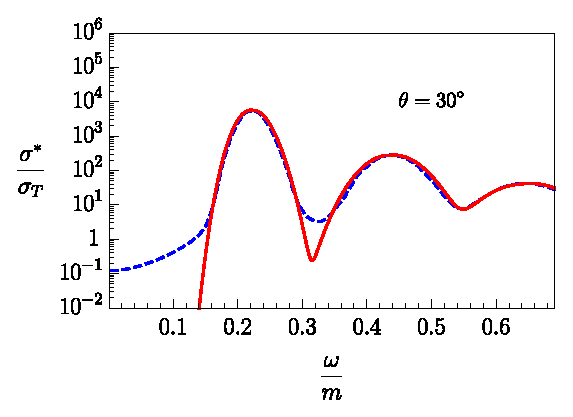
\includegraphics[width=1\linewidth,clip]{fig1_1.eps}
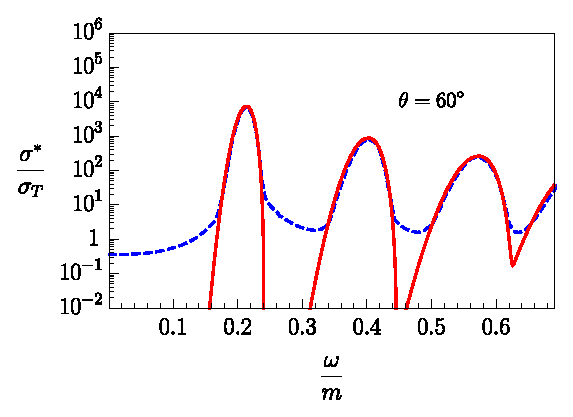
\includegraphics[width=1\linewidth,clip]{fig1_2.eps}
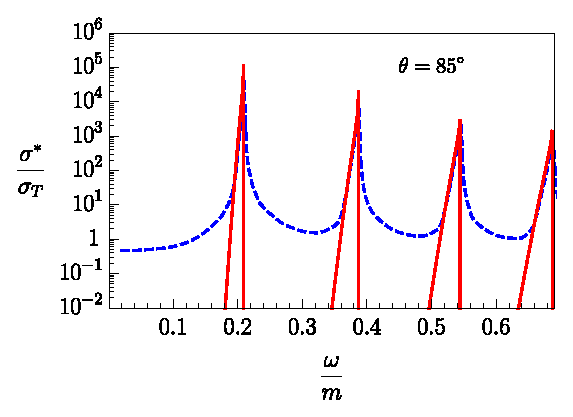
\includegraphics[width=1\linewidth,clip]{fig1_3.eps}
\caption{Зависимость усредненного по поляризациям начального фотона сечения резонансного комптоновского рассеяния, полученного в в $\delta$-функциональном приближении (сплошная линия) и с учетом конечной ширины изменения состояния электрона~\cite{Harding:1991} (пунктирная линия), от энергии начального фотона для магнитного поля $B = 10^{13}$ Гс и температуры $T=5$ кэВ для различных углов $\theta$ между импульсом фотона и направлением магнитного поля.}
\label{fig1}
\end{figure}
\begin{figure}[t!]\centering
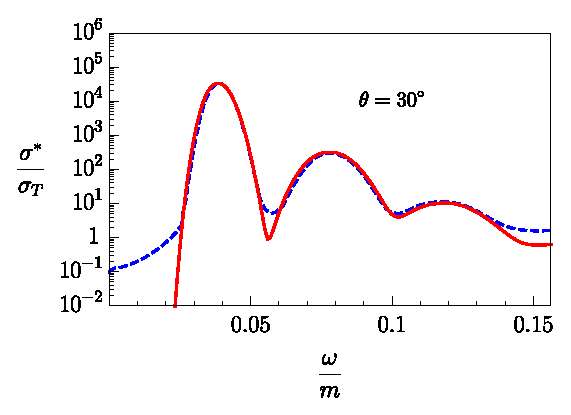
\includegraphics[width=1\linewidth,clip]{fig2_1.eps}
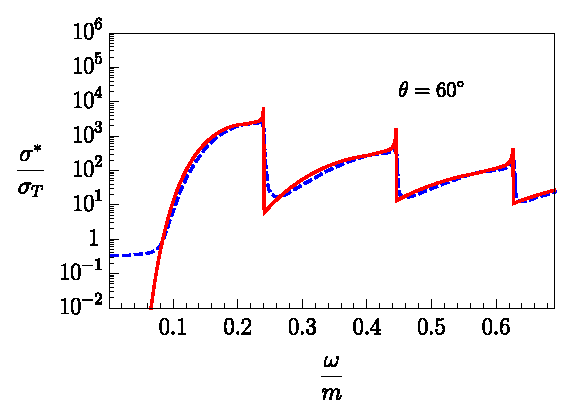
\includegraphics[width=1\linewidth,clip]{fig2_2.eps}
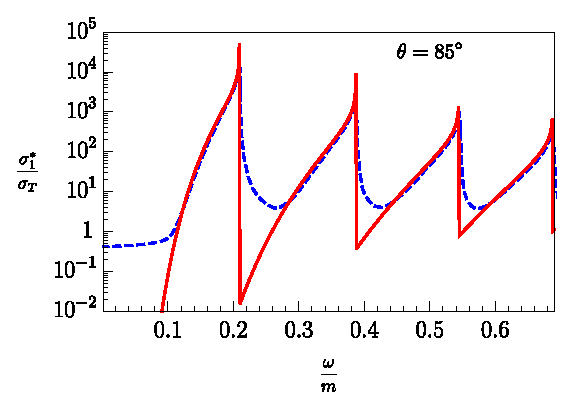
\includegraphics[width=1\linewidth,clip]{fig2_3.eps}
\caption{То же, что на рис.~\ref{fig1}, для магнитного поля $B = 10^{13}$ Гс и температуры $T=50$ кэВ.}
\label{fig2}
\end{figure}
%\clearpage

\begin{figure}[t!]\centering
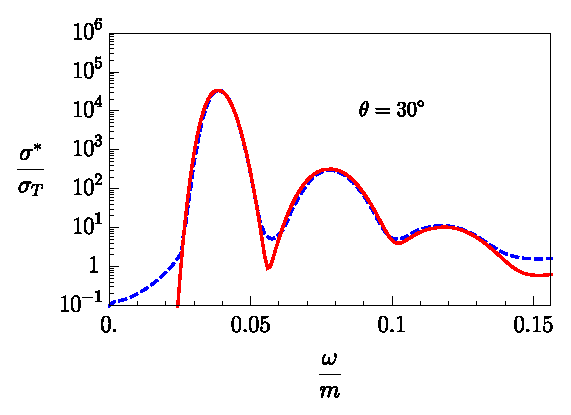
\includegraphics[width=0.99\linewidth,clip]{fig3_1.eps}
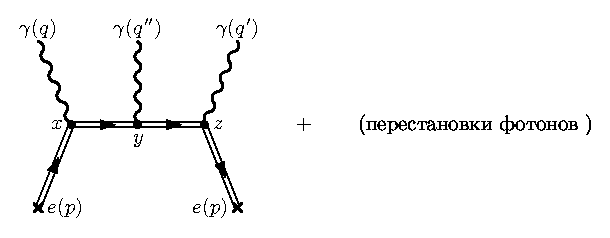
\includegraphics[width=0.99\linewidth,clip]{fig3_2.eps}
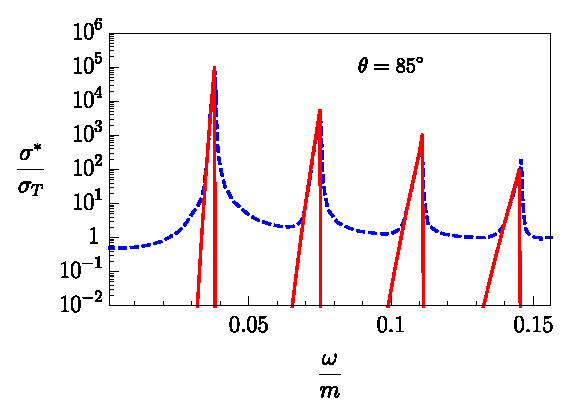
\includegraphics[width=0.99\linewidth,clip]{fig3_3.eps}
\caption{То же, что на рис.~\ref{fig1}, для магнитного поля $B = 1.7 \cdot 10^{12}$ Гс и температуры $T=5$ кэВ.}
\label{fig3}
\end{figure}
\noindent
\begin{figure}[t!]\centering
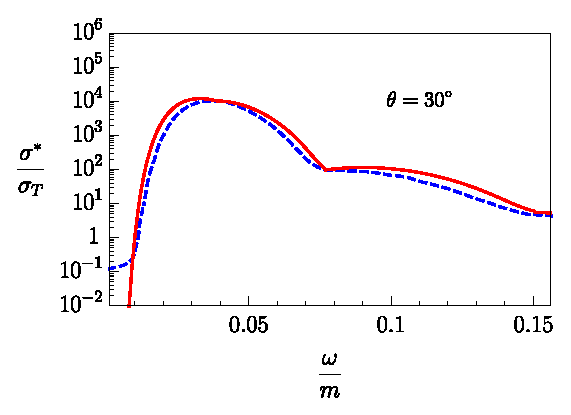
\includegraphics[width=0.99\linewidth,clip]{fig4_1.eps}
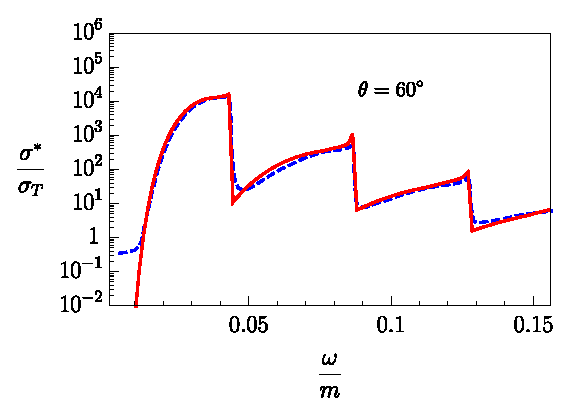
\includegraphics[width=0.99\linewidth,clip]{fig4_2.eps}
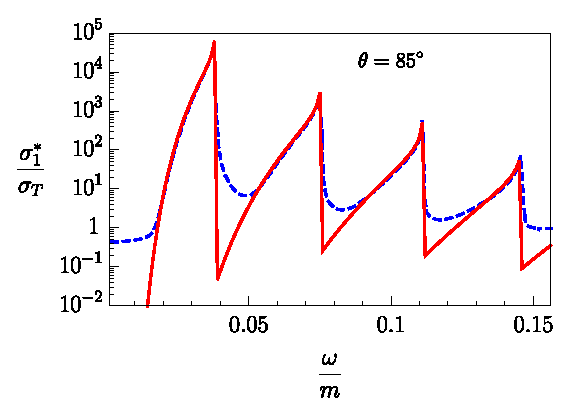
\includegraphics[width=0.99\linewidth,clip]{fig4_3.eps}
\caption{То же, что на рис.~\ref{fig1}, для магнитного поля $B = 1.7 \cdot 10^{12}$ Гс и температуры $T=50$ кэВ.}
\label{fig4}
\end{figure}
%\clearpage
%%%%%%%%%%%%%%%%%%%%%%%%%%%%%%%%%%%%%%%%%%%%%%%%%%%%%%%%%%%%%%%%%%%%%%%%%%%%%%%%%%%%%%%%%%%%%%%%%%%%%%%%%%%%%%%%%%%%%%%%%%%%%%%%%%%%%%%%%%%%%%%%%%%%%%%%%%%

\section{Резонансное комптоновское рассеяние в сверхсильных магнитных полях}
%
Рассмотрим теперь ситуацию сверхсильного магнитного поля, \mbox{$B\sim 
10^{15}-10^{16}$} Гс, и высоких температур, $T\sim 1$ МэВ, которые характерны 
для гигантских вспышек SGR -- источников мягких повторяющихся гамма-всплесков (см., например, обзор~\cite{Kaspi:2017} и цитированные в нем работы). 
Исследование комптоновского процесса в магнитных полях указанного масштаба было 
проведено, например, в работе~\cite{Chistyakov:2009}. Однако полученные в этом 
исследовании результаты будут справедливыми только для области энергий фотонов 
вдали от резонансов. Поэтому представляет самостоятельный интерес вычислить 
коэффициент поглощения фотона в пределе сильного поля с учетом возможного 
резонанса на виртуальном электроне с конечной шириной резонансного пика и 
сравнить с нерезонансным пределом~\cite{Chistyakov:2009} и 
дельта-функциональным приближением~\cite{Rumyantsev:2017}. По той причине, что в пределе 
сильного магнитного поля начальный и конечный электроны будут преимущественно 
занимать основной уровень Ландау, а виртуальный электрон -- первый уровень 
Ландау, то коэффициент поглощения фотона с учетом конечной ширины резонансного 
пика примет достаточно простой для вычисления вид. Поскольку в сильном 
магнитном поле энергии фотона, на которых наблюдается резонанс, 
выше, чем порог рождения $e^+e^-$ пары $q_{\mprl}^2=4m^2$ для фотона моды 2 , 
то целесообразно рассмотреть только каналы рассеяния $e\gamma^{(1)}\to 
e\gamma^{(1)}$ и $e\gamma^{(1)}\to e\gamma^{(2)}$. Следует отметить, что для 
фотона моды~1 порог рождения $e^+e^-$ пары $q_{\mprl}^2=(M_1+m)^2$ заведомо 
выше рассматриваемой области резонанса $q_{\mprl}^2=(M_1-m)^2$.

Как показывает численный анализ, в 
случае сильно замагниченной, горячей, зарядово-симметричной плазмы полная 
ширина поглощения электрона для первого уровня Ландау $\Gamma_1$ мало отличается от соответствующего 
выражения в 
сильном магнитном поле и ультрарелятивистских электронов~\cite{KM_Book_2013}:
\begin{equation}
	\begin{aligned}
		E''_1\Gamma_1=\alpha \beta
		(1-e^{-1})\simeq 0.623 \alpha \beta\, .
	\end{aligned}
\end{equation}

В пределе сильного поля парциальные коэффициенты поглощения фотона для каналов $e \gamma^{(1)} \to 
 e\gamma^{(1)}$ и $e \gamma^{(1)} \to e\gamma^{(2)}$ с учетом конечной ширины 
 поглощения электрона в случае, когда начальный фотон 
 распространяется поперек магнитного поля, можно 
 представить следующим образом:

\begin{strip}
%\begin{align}
%\label{Wres}
%&W_{e\gamma^{(1)}\to e\gamma^{(1)}}=\frac{\beta\alpha^2m^2}{\pi} \int 
%		dQ_0dk'_z \frac{{k_z'}^2\omega } 
%		{(-Q_{\mprl}^2)^2\varkappa}
		%\times\\&\times
%		\exp\left[-\frac{q_\perp^2+{q'}_\perp^2}{2\beta}\right]
%		\sum_{n=1}^{\infty}\sum_{\sigma=\pm 1}\frac{1}{[(n-1)!]^2}
%		\times		\\ \nonumber
%		&\times\left(\frac{\sqrt{q_\perp^2} \sqrt{q_\perp'^2}}{2\beta}\right)^{2(n-1)}\bigg\{
%		\frac{1}{((p_\sigma+q)_{\mprl}^2-M_n^2)^2+(E''_n\Gamma_n)^2}  +
%		%\\		&+
%		\frac{1}{((p_\sigma-q')_{\mprl}^2-M_n^2)^2+(E''_n\Gamma_n)^2}-
%		\\
%		\nonumber
%		&-2
%		\sum_{n'=1}^{\infty}\frac{(n-1)!}{(n'-1)!}\left(\frac{\sqrt{q_\perp^2} \sqrt{q_\perp'^2}}{2\beta}\right)^{n'+n}J_{n+n'}\left(\frac{\sqrt{q_\perp^2} \sqrt{q_\perp'^2}}{\beta}\right)\times\\
%		\nonumber
%		&\times\frac{[(p_\sigma+q)^2_{\mprl}-M_n^2][(p_\sigma-q')^2_{\mprl}-M^2_{n'}]+E''_n\Gamma_nE''_{n'}\Gamma_{n'}}{[((p_\sigma-q')_{\mprl}^2-M_n^2)^2+(E''_n\Gamma_n)^2][((p_\sigma+q)_{\mprl}^2-M_{n'}^2)^2+(E''_n\Gamma_{n'})^2]}
%		\bigg\}\times
%		\\[3mm]
%		\nonumber&\times 
%		f_e{(E_\sigma)}\left[1-f_e{(E_\sigma+Q_0)}\right]\left[1+f_\gamma(\omega')\right]
%		 \, ,
%\end{align}
%%%%%%%%%%%%%%%%%%%%%%%%%%%%%%%%%
%\begin{align}
%\label{Wres2}
%		&W_{e\gamma^{(1)}\to e\gamma^{(2)}}=\frac{\beta\alpha^2m^2}{\pi} \int 
%		dQ_0dk'_z \frac{q_\perp'^2\omega } 
%		{(-Q_{\mprl}^2)^2\varkappa}\exp\left[-\frac{q_\perp^2+{q'}_\perp^2}{2\beta}\right]
%		\times
%		\\
%		\nonumber&\times\sum_{n=1}^{\infty}\sum_{\sigma=\pm 
%		1}\frac{1}{[(n-1)!]^2}\left(\frac{\sqrt{q_\perp^2} 
%		\sqrt{q_\perp'^2}}{2\beta}\right)^{2(n-1)}\frac{Q_0}{\omega}\bigg\{
%		\frac{1}{((p_\sigma+q)_{\mprl}^2-M_n^2)^2+(E''_n\Gamma_n)^2}+
%		\\
%		\nonumber&+\frac{Q_0 \omega}{ q'^2_{\mprl}}\frac{1}{((p_\sigma-q')_{\mprl}^2-M_n^2)^2+(E''_n\Gamma_n)^2}-
%		\\
%		\nonumber&-2
%		\sum_{n'=1}^{\infty}\frac{(n-1)!}{(n'-1)!}\left(\frac{\sqrt{q_\perp^2} \sqrt{q_\perp'^2}}{2\beta}\right)^{n'+n} J_{n+n'}\left(\frac{\sqrt{q_\perp^2} \sqrt{q_\perp'^2}}{\beta}\right)\times\\
%		\nonumber&\times\frac{[(p_\sigma+q)^2_{\mprl}-M_n^2][(p_\sigma-q')^2_{\mprl}-M^2_{n'}]+E''_n\Gamma_nE''_{n'}\Gamma_{n'}}{[((p_\sigma-q')_{\mprl}^2-M_n^2)^2+(E''_n\Gamma_n)^2][((p_\sigma+q)_{\mprl}^2-M_{n'}^2)^2+(E''_n\Gamma_{n'})^2]}
%		\times\\\nonumber&\times
%		\frac{Q_0(\omega-Q_0)}{q'^2_\perp}
%		\bigg\}f_e{(E_\sigma)}\left[1-f_e{(E_\sigma+Q_0)}\right]\left[1+f_\gamma(\omega')\right]
%		 \, ,
%\end{align}
%%%%%%%%%%%%%%%%%%%%%%%%%%%%%%%%%
%\newpage
\begin{align}\label{Wresalt}
		&W_{e\gamma^{(1)}\to e\gamma^{(1)}}=\frac{\beta\alpha^2m^2}{\pi} \int 
		dQ_0dq'_z \frac{{q_z'}^2\omega } 
		{(-Q_{\mprl}^2)^2\varkappa}\exp\left[-\frac{q_\perp^2+{q'}_\perp^2}{2\beta}\right]\times
		\\
		\nonumber&\times\sum_{\sigma=\pm 1}\bigg\{
		\frac{1}{((p_\sigma+q)_{\mprl}^2-M_1^2)^2+(E''_1\Gamma_1)^2}  +\frac{1}{((p_\sigma-q')_{\mprl}^2-M_1^2)^2+(E''_1\Gamma_1)^2}-
		\\
		\nonumber&-2
		\frac{q_\perp^2 q_\perp'^2}{4\beta^2}J_{2}\left(\frac{\sqrt{q_\perp^2} \sqrt{q_\perp'^2}}{\beta}\right)\times\\
		\nonumber&\times\frac{[(p_\sigma+q)^2_{\mprl}-M_1^2][(p_\sigma-q')^2_{\mprl}-M^2_{1}]+(E''_1\Gamma_{1})^2}{[((p_\sigma-q')_{\mprl}^2-M_1^2)^2+(E''_1\Gamma_1)^2][((p_\sigma+q)_{\mprl}^2-M_{1}^2)^2+(E''_1\Gamma_{1})^2]}
		\bigg\}\times
		\\\nonumber&\times 
		f_e{(E_\sigma)}\left[1-f_e{(E_\sigma+Q_0)}\right]\left[1+f_\gamma(\omega')\right]
		\, ,
	\end{align}
%%%%%%%%%%%%%%%%%%%%%%%%%%%%%%%%%
\begin{align}\label{Wres2alt}
		&W_{e\gamma^{(1)}\to e\gamma^{(2)}}=\frac{\beta\alpha^2m^2}{\pi} \int 
		dQ_0dq'_z \frac{q_\perp'^2\omega } 
		{(-Q_{\mprl}^2)^2\varkappa}\exp\left[-\frac{q_\perp^2+{q'}_\perp^2}{2\beta}\right]
		\times
		\\
		\nonumber&\times\sum_{\sigma=\pm 
			1}\frac{Q_0}{\omega}\bigg\{
		\frac{1}{((p_\sigma+q)_{\mprl}^2-M_1^2)^2+(E''_1\Gamma_1)^2}+\frac{Q_0 \omega}{ q'^2_{\mprl}}\frac{1}{((p_\sigma-q')_{\mprl}^2-M_1^2)^2+(E''_1\Gamma_1)^2}-
		\\
		\nonumber&-2
		\frac{q_\perp^2 q_\perp'^2}{4\beta^2} J_{2}\left(\frac{\sqrt{q_\perp^2} \sqrt{q_\perp'^2}}{\beta}\right)\times\\
		\nonumber&\times\frac{[(p_\sigma+q)^2_{\mprl}-M_1^2][(p_\sigma-q')^2_{\mprl}-M^2_{1}]+(E''_1\Gamma_1)^2}{[((p_\sigma-q')_{\mprl}^2-M_1^2)^2+(E''_1\Gamma_1)^2][((p_\sigma+q)_{\mprl}^2-M_{1'}^2)^2+(E''_1\Gamma_{1'})^2]}
		\times\\\nonumber&\times
		\frac{Q_0(\omega-Q_0)}{q'^2_\perp}
		\bigg\}f_e{(E_\sigma)}\left[1-f_e{(E_\sigma+Q_0)}\right]\left[1+f_\gamma(\omega')\right]
		\, ,
\end{align}
\end{strip}

\noindent где $J_n(x)$ -- функция Бесселя целого индекса, 
\mbox{$\varkappa = \sqrt{1 - 4m^2/Q^2_{\mprl}}$, 
	$E_\sigma=\sqrt{p_{z\sigma}^2+m^2}$}, $p_{z\sigma}$ -- корни уравнения 
$Q_0+E_\sigma-E'_\sigma=0$:
\begin{equation}\label{savelaw}
	p_{z\sigma}=-\frac{Q_z}{2}+ \sigma Q_0 \varkappa\, ,
\end{equation}
$p^\alpha_{\sigma\mprl}=(E_\sigma,p_{z\sigma})$. 
Поперечная составляющая импульса конечного фотона определяется из уравнения 
дисперсии (см.~\cite{Chistyakov:2009}):
\begin{equation}
	q'^2_{\mprl}=q'^{2}_\perp + {\cal P}^{(\lambda)}(q') .
\end{equation}

Имеет смысл провести сравнительный анализ результатов работы~\cite{Chistyakov:2009}  с резонансным случаем (\ref{Wresalt}) и (\ref{Wres2alt}) для зарядово-симметричной плазмы и поперечного направления распространения импульса фотона по отношению к внешнему магнитному полю для различных значений величины магнитного поля, температуры и энергии начального фотона.

На рис.~\ref{fig5}--\ref{fig8} показаны коэффициенты поглощения для каналов $\gamma^{(1)}e\to\gamma^{(1)}e$ и $\gamma^{(1)}e\to\gamma^{(2)}e$ при температуре $T=1 $~МэВ и величине магнитного поля $B=200B_e$ и $B=20B_e$ соответственно. Как видно из рис.~\ref{fig5}--\ref{fig6}, коэффициент поглощения для канала $\gamma^{(1)}e\to\gamma^{(1)}e$ согласуется с погрешностью не более 8\% с соответствующими результатами для предела сильного поля и отсутствия резонанса, полученными в работе \cite{Chistyakov:2009}, вплоть до энергий начального фотона  $\omega\simeq3$~МэВ для поля $B=200B_e$ и  $\omega\simeq0.3$~МэВ для поля $B=20B_e$ . Отсюда вытекает ограничение на применимость результатов работы \cite{Chistyakov:2009} по энергиям начального фотона. Аналогичная ситуация наблюдается и для канала $\gamma^{(1)}e\to\gamma^{(2)}e$ (см. рис. \ref{fig7}--\ref{fig8}), для которого точность соответствия с коэффициентом поглощения в нерезонансном пределе -- до 16\% для значений магнитных полей $B=200B_e$ и до 18\% для значений магнитных полей $B=20B_e$ в нерезонансной области.  На рис. \ref{fig6} и \ref{fig8} наиболее ярко видно завышение коэффициента поглощения даже при относительно малых энергиях начального фотона. Этот факт связан с тем, что в пределе сильного магнитного поля разложение амплитуды комптоновского процесса по обратным степеням поля уже не будет правомочным.

С  другой стороны, $\delta$-функциональное приближение достаточно хорошо описывает первый резонансный пик. Действительно, для канала $\gamma^{(1)}e\to\gamma^{(1)}e$ погрешность в пределе узкого резонансного пика с составляет не более 9\% для значения магнитного поля $B=200B_e$ и 13\% для $B=20 B_e$. Учет дисперсии фотона моды 2 для канала $\gamma^{(1)}e\to\gamma^{(2)}e$ приводит к более высокому несоответствию -- до 15\% для $B=200B_e$ и до 25\% для $B=20B_e$.
Следует отметить   что при относительно малых температурах $T\lesssim50$ кэВ и магнитных полях той же величины ($B = 200 B_e$ и $B = 20 B_e$) $\delta$-аппроксимация работает хуже из-за уменьшения области резонанса по энергии фотона. В целом $\delta$-функциональное приближение достаточно хорошо будет описывать лишь первый резонансный пик.

\begin{figure}[h]\centering
	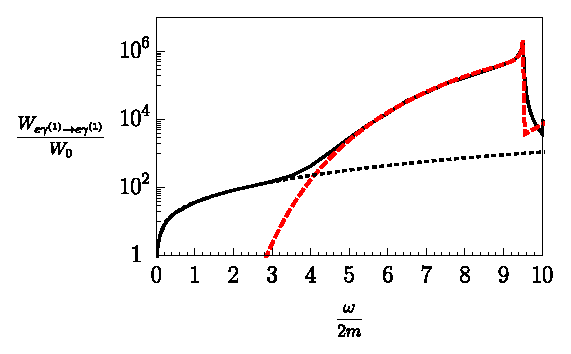
\includegraphics[width=0.9\linewidth]{fig5.eps}
	\caption{Зависимость коэффициента поглощения от энергии начального фотона для канала $e\gamma^{(1)}\to e\gamma^{(1)}$ при поле $B=200 B_e$ и температуре T=1 МэВ: сплошная линия -- коэффициент поглощения с учетом резонанса; штриховая линия -- без учета резонанса; пунктирная линия -- дельта-функциональное приближение. Здесь $W_0=(\alpha/\pi)^3m\simeq 3.25\cdot10^2$ см$^{-1}$.}
	\label{fig5}
\end{figure}
\begin{figure}[h]\centering
	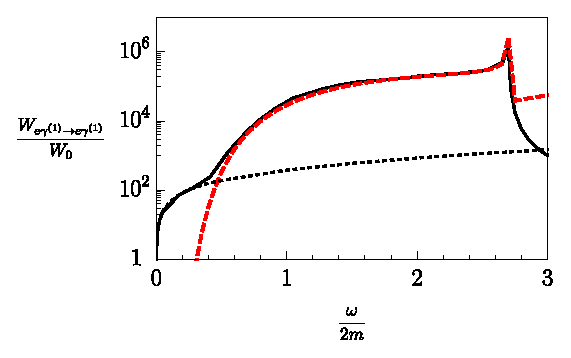
\includegraphics[width=0.9\linewidth]{fig6.eps}
	\caption{Зависимость коэффициента поглощения от энергии начального фотона для канала $e\gamma^{(1)}\to e\gamma^{(1)}$ при поле $B=20 B_e$ и температуре T=1 МэВ. Обозначение для линий то же, что и для рис. \ref{fig5}.}
	\label{fig6}
\end{figure}
\begin{figure}[h]\centering
	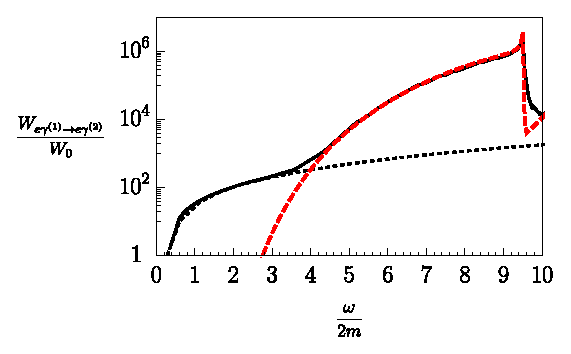
\includegraphics[width=0.9\linewidth]{fig7.eps}
	\caption{Зависимость коэффициента поглощения от энергии начального фотона для канала $e\gamma^{(1)}\to e\gamma^{(2)}$ при поле $B=200 B_e$ и температуре T=1 МэВ. Обозначение для линий то же, что и для рис. \ref{fig5}.}
	\label{fig7}
\end{figure}
\begin{figure}[h]\centering
	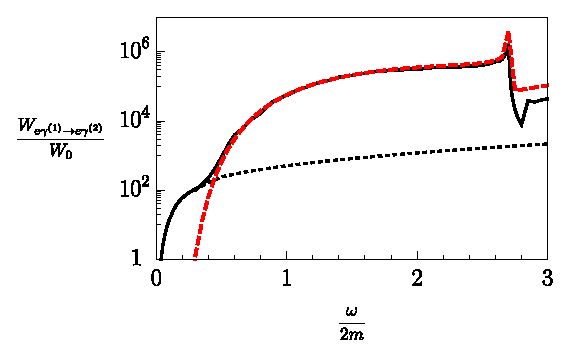
\includegraphics[width=0.9\linewidth]{fig8.eps}
	\caption{Зависимость коэффициента поглощения от энергии начального фотона для канала $e\gamma^{(1)}\to e\gamma^{(2)}$ при поле $B=20 B_e$ и температуре T=1 МэВ. Обозначение для линий то же, что и для рис. \ref{fig5}.}
	\label{fig8}
\end{figure}


%%%%%%%%%%%%%%%%%%%%%%%%%%%%%%%%%%%%%%%%%%%%%%%%%%%%%%%%%%%%%%%%%%%%%%%%%%%%%%%%%%%%%%%%%%%%%%%%%%%%%%%%%%%%%%%%%%%%%%%%%%%%%%%%%%%%%%%%%%%%%%%%%%%%%%%%%%%


\section{Заключение}

В данной работе вычислены коэффициенты поглощения и дифференциальное сечение в реакции комптоновского рассеяния в относительно сильном магнитном поле $B\gtrsim B_e$ в приближении узкого резонансного пика. Показано, что такое приближение дает хорошее согласие с результатами более ранних работ~\cite{Harding:1991,Mushtukov:2015,SchwarmD:2017}.

В пределе сильного магнитного поля $B\gg B_e$ и высоких температур $T=1$ МэВ вычислен коэффициент поглощения фотона в комптоновском процессе для двух кинематически разрешенных каналов $\gamma^{(1)} e\to \gamma^{(1)} e$ и $\gamma^{(1)} e\to \gamma^{(2)} e$ . Полученные численные результаты позволили установить области энергий фотона, при которых применим нерезонансный предел, использованный в работе~\cite{Chistyakov:2009}: $\omega\lesssim 3$ МэВ при $B=200B_e$ и $\omega\lesssim 0.3$ МэВ при $B=20B_e$. Показано, чтодельта-функциональное приближение при данных параметрах среды хорошо описывает только первый резонансный пик.



\section*{Приложение. Амплитуда поглощения фотона}

Входящие в выражение~(\ref{eq:amplonever}) величины ${\cal T}^{s'' s}_\lambda$ выражаются через следующие 
лоренц-инварианты:
%
\begin{eqnarray}
\label{eq:K1}
&&{\cal K}_{1}^{(\lambda)} = \sqrt{\frac{2}{(p\tilde \varphi\tilde \varphi p^{\, \prime \prime}) + 
M_\ell M_{n}}} \times 
\\
\nonumber 
&&\times \left \{M_\ell (\varepsilon^{(\lambda)}\tilde \varphi\tilde \varphi p^{\, \prime \prime}) + 
M_{n} (\varepsilon^{(\lambda)}\tilde \varphi\tilde \varphi p)  \right \}\, ,
\end{eqnarray}
%
\begin{eqnarray}
&&{\cal K}_{2}^{(\lambda)} = \sqrt{\frac{2}{(p\tilde \varphi\tilde \varphi p^{\, \prime \prime}) + 
M_\ell M_{n}}} 
\times
\\
\nonumber
&&\times
 \left \{M_\ell (\varepsilon^{(\lambda)}\widetilde \varphi p^{\, \prime \prime}) + 
M_{n} (\varepsilon^{(\lambda)}\widetilde \varphi p)  \right \}\, ,
\label{eq:K2}
\end{eqnarray}
%
\begin{eqnarray}
{\cal K}_{3} = \sqrt{2\left [(p\tilde \varphi\tilde \varphi p^{\, \prime \prime}) + 
M_\ell M_{n} \right]} \, ,  
\end{eqnarray}
%
\begin{eqnarray}
{\cal K}_4 = 
- \sqrt{\frac{2}{(p\tilde \varphi\tilde \varphi p^{\, \prime \prime}) + M_\ell M_{n}}}\, 
(p\widetilde \varphi p^{\, \prime \prime}) \, ,
\label{eq:K34}
\end{eqnarray}
%

Выражения для ${\cal T}^{s'' s}_\lambda$ представлены ниже:
%
\begin{eqnarray}
\nonumber
&&{\cal T}^{--}_\lambda  = e [ 2\beta\sqrt{\ell n} {\cal K}_1^{(\lambda)} I_{n-1,\ell-1} +
\\[3mm]
\label{eq:tV--}
&&+ (M_\ell + m)(M_n + m) {\cal K}_1^{(\lambda)} I_{n,\ell} -
\\[3mm]
\nonumber
%transversal
&&-\sqrt{2\beta n} (M_\ell + m) {\cal K}_3 \times
\\[3mm]
\nonumber
&&\times\frac{(\varepsilon^{(\lambda)}\varphi\varphi q) - 
\ii (\varepsilon^{(\lambda)} \varphi q)}{\sqrt{q^2_{\mprp}}} I_{n-1,\ell} -
\\[3mm]
\nonumber
&&- \sqrt{2\beta \ell} (M_n + m) {\cal K}_3 \times
\\[3mm]
\nonumber
&&\times
\frac{(\varepsilon^{(\lambda)}\varphi\varphi q) + \ii (\varepsilon^{(\lambda)}\varphi q)}{\sqrt{q^2_{\mprp}}} I_{n,\ell-1}] \, ,
\end{eqnarray}



\begin{eqnarray}
\nonumber
&&{\cal T}^{-+}_\lambda = \ii e [\sqrt{2\beta n} (M_\ell + m) {\cal K}_2^{(\lambda)} 
I_{n-1,\ell-1} - 
\\[3mm]\nonumber
&&- \sqrt{2\beta \ell} (M_n + m) {\cal K}_2^{(\lambda)} 
I_{n,l} +
\\[3mm]
\nonumber
%transversal
&&+ 2\beta\sqrt{\ell n} {\cal K}_4 
\frac{(\varepsilon^{(\lambda)}\varphi\varphi q) - \ii (\varepsilon^{(\lambda)}\varphi q)}{\sqrt{q^2_{\mprp}}} I_{n-1,\ell} -
\nonumber\\[3mm]
&&- (M_\ell + m)(M_n + m) {\cal K}_4 \times
\\[3mm]
\nonumber
&&\times
\frac{(\varepsilon^{(\lambda)}\varphi\varphi q) + \ii (\varepsilon^{(\lambda)}\varphi q)}{\sqrt{q^2_{\mprp}}} I_{n,\ell-1}]  \, ,
\nonumber
\end{eqnarray}

\begin{eqnarray}
&&{\cal T}^{+-}_\lambda = -\ii e [\sqrt{2\beta \ell} (M_n + m) {\cal K}_2^{(\lambda)} 
I_{n-1,\ell-1} - 
\nonumber\\[3mm]
&&- \sqrt{2\beta n} (M_\ell + m) {\cal K}_2^{(\lambda)} 
I_{n,\ell} +
\\[3mm]
\nonumber
%transversal
&&+ (M_\ell + m)(M_n + m) {\cal K}_4 \times
\\[3mm]
\nonumber
&&\times
\frac{(\varepsilon^{(\lambda)}\varphi\varphi q) - \ii (\varepsilon^{(\lambda)}\varphi q)}{\sqrt{q^2_{\mprp}}} I_{n-1,\ell} -
\nonumber\\[3mm]
&&- 2\beta\sqrt{\ell n} {\cal K}_4 
\frac{(\varepsilon^{(\lambda)}\varphi\varphi q) + \ii (\varepsilon^{(\lambda)}\varphi q)}{\sqrt{q^2_{\mprp}}} I_{n,\ell-1}]  \, ,
\nonumber
\end{eqnarray}

\begin{eqnarray}
\nonumber
&&{\cal T}^{++}_\lambda  = e [2\beta\sqrt{\ell n} {\cal K}_1^{(\lambda)} I_{n,\ell} +
\\[3mm]
\label{eq:tV++} 
&&+ (M_\ell + m)(M_n + m) {\cal K}_1^{(\lambda)} I_{n-1,\ell-1} -
\\[3mm]
\nonumber
%transversal
&&- \sqrt{2\beta \ell} (M_n + m) {\cal K}_3 \times
\\[3mm]
\nonumber
&&\times
\frac{(\varepsilon^{(\lambda)}\varphi\varphi q) - \ii (\varepsilon^{(\lambda)}\varphi q)}{\sqrt{q^2_{\mprp}}} I_{n-1,\ell} -
\\[3mm]
\nonumber
&&- \sqrt{2\beta n} (M_\ell + m) {\cal K}_3 \times
\\[3mm]
\nonumber
&&\times
\frac{(\varepsilon^{(\lambda)}\varphi\varphi q) + \ii (\varepsilon^{(\lambda)}\varphi q)}{\sqrt{q^2_{\mprp}}} I_{n,\ell-1}] \, .
\end{eqnarray}

%%%%%%%%%%%%%%%%%%%%%%%%%%%%%%%%%%%%%%%%%%%%%%%%%%%%%%%%%%%%%%%%%%%%%%%%
%% Библиография %%%%%%%%%%%%%%%%%%%%%%%%%%%%%%%%%%%%%%%%%%%%%%%%%%%%%%%%
%%%%%%%%%%%%%%%%%%%%%%%%%%%%%%%%%%%%%%%%%%%%%%%%%%%%%%%%%%%%%%%%%%%%%%%%

\begin{references}
%
\bibitem{Truemper1978}
 Tr\"{u}mper~J., Pietsch~W., Reppin~C., Voges~W., Staubert~R., Kendziorra~E., Astrophys. J. {\bf 219}, L105 (1978).
  
%
\bibitem{Makishima1990}
  Makishima~K., Mihara~T., Ishida~M. et al., Astrophys. J. Lett. {\bf 365}, L59 (1990).
%
\bibitem{Grove1995}
  Grove~J.~E., Strickman~M.~S., Johnson~W.~N. et al., Astrophys. J. Lett. {\bf 438}, L25 (1995).
%
\bibitem{Mihara:1990}
  Mihara~T., Makishima~K., Ohashi~T., Sakao~T., Tashiro~M., Nagase~F., Tanaka~Y., Kitamoto~S., Miyamoto~S., Deeter~J.~E., 
  Boynton~P.~E., Nature {\bf 346}, 250 (1990).
%
\bibitem{Canuto:1971}
Canuto~V., Lodenquai~J., Ruderman~M., Phys. Rev. D {\bf 3}, 2303 (1971).
%
\bibitem{Gnedin1973}
    Гнедин~Ю.~Н., Сюняев~Р.~А., ЖЭТФ {\bf 65}, 102 (1973).
%
\bibitem{Borner1979}
  Borner~G., Meszaros~P., Plasma Phys. {\bf 21}, 357 (1979).
%
\bibitem{Ventura:1979}
  Ventura~J., Phys. Rev. D {\bf 19}, 1684 (1979).

%
\bibitem{Herold:1979}
   Herold~H., Phys. Rev. D {\bf 19}, 2868 (1979).
%
\bibitem{Melrose:1983III}
  Melrose~D.~B., Parle~ A.~J.,
   Aust.~J.~Phys. {\bf 36}, 799 (1983).

%
\bibitem{Daugherty:1986}
  Daugherty~J.~K., Harding~A.~K., Astrophys. J. {\bf 309}, 362 (1986).
%
\bibitem{Bussard:1986}
Bussard~R.~W., Alexander~S.~B., Meszaros~P., Phys. Rev. D {\bf 34}, 440 (1986).
%
\bibitem{Ozel:2001}
  {\"O}zel~F., Astrophys. J. {\bf 563}, 276 (2001).
%
\bibitem{Zavlin:1996}
  Zavlin~V.~E., Pavlov~G.~G., Shibanov~Yu.~A., A\&A {\bf 315}, 141 (1996).
%
\bibitem{Alexander:1991}
   Alexander~S.~G., Meszaros~P.,  Astrophys. J. {\bf 372}, 565 (1991).
%
\bibitem{Araya:1999}
  Araya~R.~A., Harding~A.~K.,  Astrophys. J. {\bf 517}, 334 (1999).
%
\bibitem{Ho:2001}
  Ho~W.~C.~G., Lai~D., MNRAS, {\bf 327}, 1081 (2001).
%
\bibitem{Lyutikov:2006}
   Lyutikov~M., Gavriil~F.~P., MNRAS, {\bf 368}, 690 (2006).
%
\bibitem{Potekhin:2004}
  Potekhin~A.~Y., Lai~D., Chabrier~G., Ho~W.~C.~G., Astrophys. J. {\bf 621}, 1034 (2004).
%
\bibitem{Schonherr:2007}
   Sch{\"o}nherr~G., Wilms~J., Kretschmar~P., Kreykenbohm~I., Santangelo~A., Rothschild~R.~E., Coburn~W., Staubert~R., 
   A{\&}A {\bf 472}, 353 (2007).
%
\bibitem{Nishimura:2008}
  Nishimura~O., Astrophys. J. {\bf 672}, 1127 (2008).
  %
\bibitem{Suleimanov:2009}
   Suleimanov~V., Potekhin~A.~Y., Werner~K., A{\&}A {\bf 500}, 891 (2009).
  %
\bibitem{Fernandez:2007}
   Fern{\'a}ndez~R., Thompson~C., Astrophys. J. {\bf 660}, 615 (2007).
  %
\bibitem{Nobili:2008}
Nobili~L., Turolla~R., Zane~S., MNRAS, {\bf 389}, 989 (2008).
%
\bibitem{Baring:2018}
Wadiasingh~Z., Baring~M.~G., Gonthier~P.~L., Harding~A.~K., Astrophys. J. {\bf 854}, 98 (2018).
%
\bibitem{Beloborodov:2013}
  Beloborodov~A.~M., Astrophys. J. {\bf 762}, 13 (2013).
%
\bibitem{Daugherty:1989}
  Daugherty~J.~K., Harding~A.~K., Astrophys. J. {\bf 336}, 861 (1989).
%
\bibitem{Gonthier:2000}
Gonthier~P.~L., Harding~A.~K., Baring~M.~G., Costello~R.~M., Mercer~C.~L., Astrophys. J. {\bf 540}, 1719 (2010).
%
\bibitem{Holodov:2000}
Фомин~П.~И., Холодов~Р.~И., ЖЭТФ {\bf 117}, 319 (2000). 
%
\bibitem{Gonthier:2014}
P.~L.~Gonthier, M.~G.~Baring et al., 
   Phys. Rev. D {\bf 90},  043014 (2014).

%
\bibitem{Mushtukov:2016}
Mushtukov~A.~A., Nagirner~D.~I., Poutanen~J., Phys. Rev. D {\bf 93}, 105003 (2016).
%
\bibitem{Harding:1991}
Harding~A.~K., Daugherty~J.~K., Astrophys. J. {\bf 374}, 687 (1991).
%
\bibitem{Rumyantsev:2017}
Румянцев~Д.~А., Шленев~Д.~М., Ярков~А.~А., ЖЭТФ {\bf 152}, 483 (2017). 
%
\bibitem{Sokolov:1968} 
   Sokolov~A.~A., Ternov~I.~M., {\it Synchrotron Radiation}, Pergamon: Oxford (1968).

%
\bibitem{Gradstein:1963}
Градштейн~И.~С.,  Рыжик~И.~М., {\it Таблицы интегралов, сумм, рядов и
   произведений}, Физматлит: Москва (1963). 
%
\bibitem{Chistyakov:2009}
Chistyakov~M.~V., Rumyantsev~D.~A., 
   Int.~J.~Mod.~Phys.~A {\bf 24}, 3995 (2009).
%
\bibitem{Weldon:1982}
Weldon~H.~A., Phys.~Rev.~D {\bf 26}, 1394 (1982).
%
\bibitem{Zhukovski:1994}
Жуковский~В.~Ч., Мидодашвили~П.~Г., Эминов~П.~А., ЖЭТФ {\bf 106}, 929 (1994). 
%
\bibitem{Weldon:1983}
Weldon~H.~A., Phys.~Rev.~D {\bf 28}, 2007 (1983).
%
\bibitem{Harding:1986}
Daugherty~J.~K., Harding~A.~K., Astrophys. J. {\bf 309}, 362 (1986).
%
\bibitem{Landau:2002}
Берестецкий~В.~Б., Лифшиц~Е.~М., Питаевский~Л.~П., {\it Квантовая электродникамика}, Физматлит: Москва (2002). 
%
\bibitem{SchwarmD:2017}
Schwarm~F.-W.,  Sch{\"o}nherr~G.,  Falkner~S.,  Pottschmidt~K., Wolff~M.~T., Becker~P.~A., Sokolova-Lapa~E., Klochkov~D., Ferrigno~C., F{\"u}rst~F., Hemphill~P.~B., Marcu-Cheatham~D.~M., Dauser~T., Wilms~J., A{\&}A {\bf 597}, A3 (2017).
%
\bibitem{Mushtukov:2015}
Mushtukov~A.~A., Suleimanov~V.~F., Tsygankov~.S~S., Poutanen~J., MNRAS, {\bf 447}, 1847 (2015).
%
\bibitem{Pavlov:1991}
Pavlov~G.~G., Bezchastnov~V.~G., Meszaros~P., Alexander~S.~G.,   
   Astrophys.~J. {\bf 380}, 541 (1991).
%
\bibitem{Klepikov:1954}
Клепиков~Н.~П., 
  ЖЭТФ \textbf{26}, 19 (1954).
%
\bibitem{Baier:2007}
Baier~V.~N., Katkov~V.~M., Phys.~Rev.~D {\bf 75}, 073009 (2007).

%
\bibitem{Kaspi:2017}
Kaspi~V.~M., Beloborodov~A.~M., Annu. Rev. Astron. \& Astrophys, {\bf 55}, 261 (2017).
%
\bibitem{KM_Book_2013}
Kuznetsov~A.~V., Mikheev~N.~V.,
   {\it Electroweak Processes in External Active Media}, 
   Springer-Verlag: Berlin, Heidelberg (2013).
   

\end{references}

\end{document}